% Conceptos Generales y Revisión de la Literatura

% En este capítulo debe ser proporcionado el estado del arte o referencial teórico sobre el tema al que se refiere el estudio. Un buen investigador no debe repetir trabajos ya concluidos o que ya están en marcha. Por eso esta sesión es donde el autor demuestra hasta dónde va la investigación actual en el campo de estudios en cuestión y establece las bases sobre las cuales desarrollará el estudio propuesto. También este punto se podría denominar "Situación actual de la tecnología". No se habla del estado actual de la tecnología con la que se desarrollará el trabajo, sino de qué otras aplicaciones que existen actualmente o han existido en el mercado (historia de la evolución tecnológica) y que realicen funcionalidades iguales o parecidas a las que se propone desarrollar en el TFG. En este punto hay que presentar lo que hay, simplemente describiendo. Se puede hacer alguna pequeña valoración que muestre los puntos fuertes de la tecnología o su utilidad, en que ámbitos se puede aplicar, para posteriormente, en el apartado de "Crítica al estado del arte" enjuiciar constructivamente cada aportación y de ahí extraer consecuencias para el TFG.

\chapter{Sistemas de Información Geográfica}
\label{ch:capitulo2}

\begin{quote}
  	{\bf\textsc{Resumen:}} Este capítulo presenta los SIG como una herramienta que permite manejar Información Geográfica. De esta forma, explicaremos y nos adentraremos en el mundo de los SIG, hablaremos sobre los posibles modelos y representaciones de los datos geográficos, y de algunas herramientas existentes en el mercado para el tratamiento de datos e Información Geográfica.
\end{quote}

% coger lo del TFG y modificarlo y adaptarlo un poco, y ver algún enlace nuevo  

\section{Sistemas de Información Geográfica}

A continuación, vamos a introducir la definición de SIG, para ello se va a tratar de contextualizar los elementos clave de los SIG.

% Definición de los SIG

% https://www.ceupe.com/blog/los-sistemas-de-informacion-geografica.html

\subsection{Conceptos generales}

Los \textbf{Sistemas de Información Geográfica} \textbf{(SIG)} o \textbf{GIS} \textbf{(\textit{Geographic Information System})}, hacen referencia a una amplia familia de estándares, tecnologías y herramientas de software para almacenar, editar, analizar, mostrar e integrar datos espaciales. En el presente trabajo, nos vamos a centrar mayoritariamente en los aspectos de \textit{búsqueda} e \textit{integración} \cite{tesis}. De tal forma que los SIG son sistemas complejos que integran un conjunto de elementos interrelacionados entre sí \cite{VictorOlaya} (figura \ref{fig:elementosSIG}). Sin embargo, desde otro punto de vista, un SIG consiste en la unión de dos ciencias: la Geografía y la Informática, es decir, consiste en un Sistema de Información (SI) en donde dicha información incluye su posición en el espacio, utilizando para ello un sistema de coordenadas estandarizado resultado de una proyección cartográfica. 

\begin{figure}[H]
	\centering
	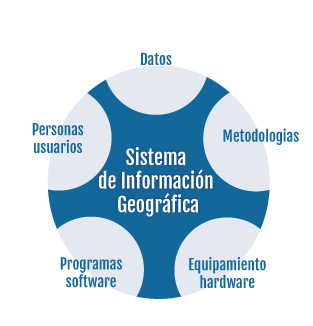
\includegraphics[width=0.49\textwidth]{imagenes/capitulo2/graficoSig}
	\caption{Elementos que conforman el sistema SIG \cite{image-capitulo2}}
	\label{fig:elementosSIG}
\end{figure}

Para trabajar con información espacial georreferenciada es necesario el establecimiento de un sistema de referencia con el que poder expresar la situación de un punto dado, es decir, se necesita establecer un sistema de codificación para cada una de las posiciones sobre la superficie terrestre y la asignación de estas a sus correspondientes coordenadas \cite{VictorOlaya}. De entre todos los posibles sistemas de referenciación que hay, nos vamos a centrar en el sistema de coordenadas \textit{UTM}, \textit{WGS84} y \textit{ETRS89}  los cuales son los sistemas usados en los datos geográficos escogidos para la realización de la prueba de concepto. Antes de entrar en detalle, es importante saber que cada país o continente usa un modelo diferente (el que mejor se aproxima a su situación), es por eso que debemos prestar especial atención a cuál se está usando. 

\begin{itemize}
	\item \textbf{UTM (\textit{Universal Transversal de Mercator})} es un sistema de proyección geodésica en el cual se construye geométricamente el mapa de manera que los meridianos y paralelos se transforman en una red rectangular, de tal forma que se conservan los ángulos pero se distorsionan todas las superficies sobre los objetos originales \cite{utm-nuevo}. En este sistema se divide al globo terráqueo en 60 zonas septentrionales y meridionales, en donde cada zona tiene su propio meridiano central. En la figura \ref{fig:UTM} podemos ver cómo es la división mundial.
	
	\item \textbf{WGS84} \textbf{(\textit{World Geodetic System 1984})} es un sistema de coordenadas geográficas mundial que permite localizar cualquier punto de la Tierra por medio de tres unidades dadas, es el más empleado en la actualidad. Este sistema de coordenadas agrega a \textit{Greenwich} como el punto de inicio (primer meridiano) para la longitud ($0^o$) y establece las unidades en grados. Además, el sistema GPS lo emplea como sistema geodésico de referencia \cite{VictorOlaya} (figura \ref{fig:WGS84}).
	
	\begin{figure}[H]
		\centering
		\begin{subfigure}[h]{0.33\textwidth} 
			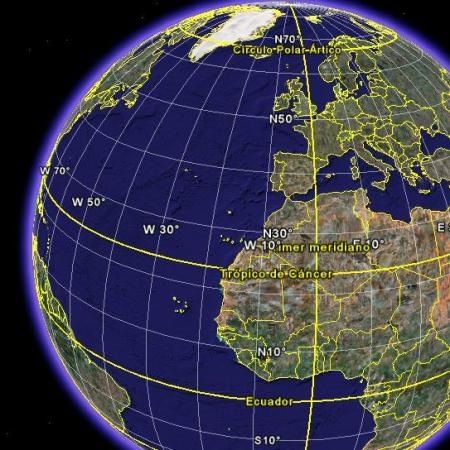
\includegraphics[width=\textwidth]{imagenes/capitulo2/2_utm1.jpg}
			\caption{}
		\end{subfigure}       
		\begin{subfigure}[h]{0.636\textwidth} 
			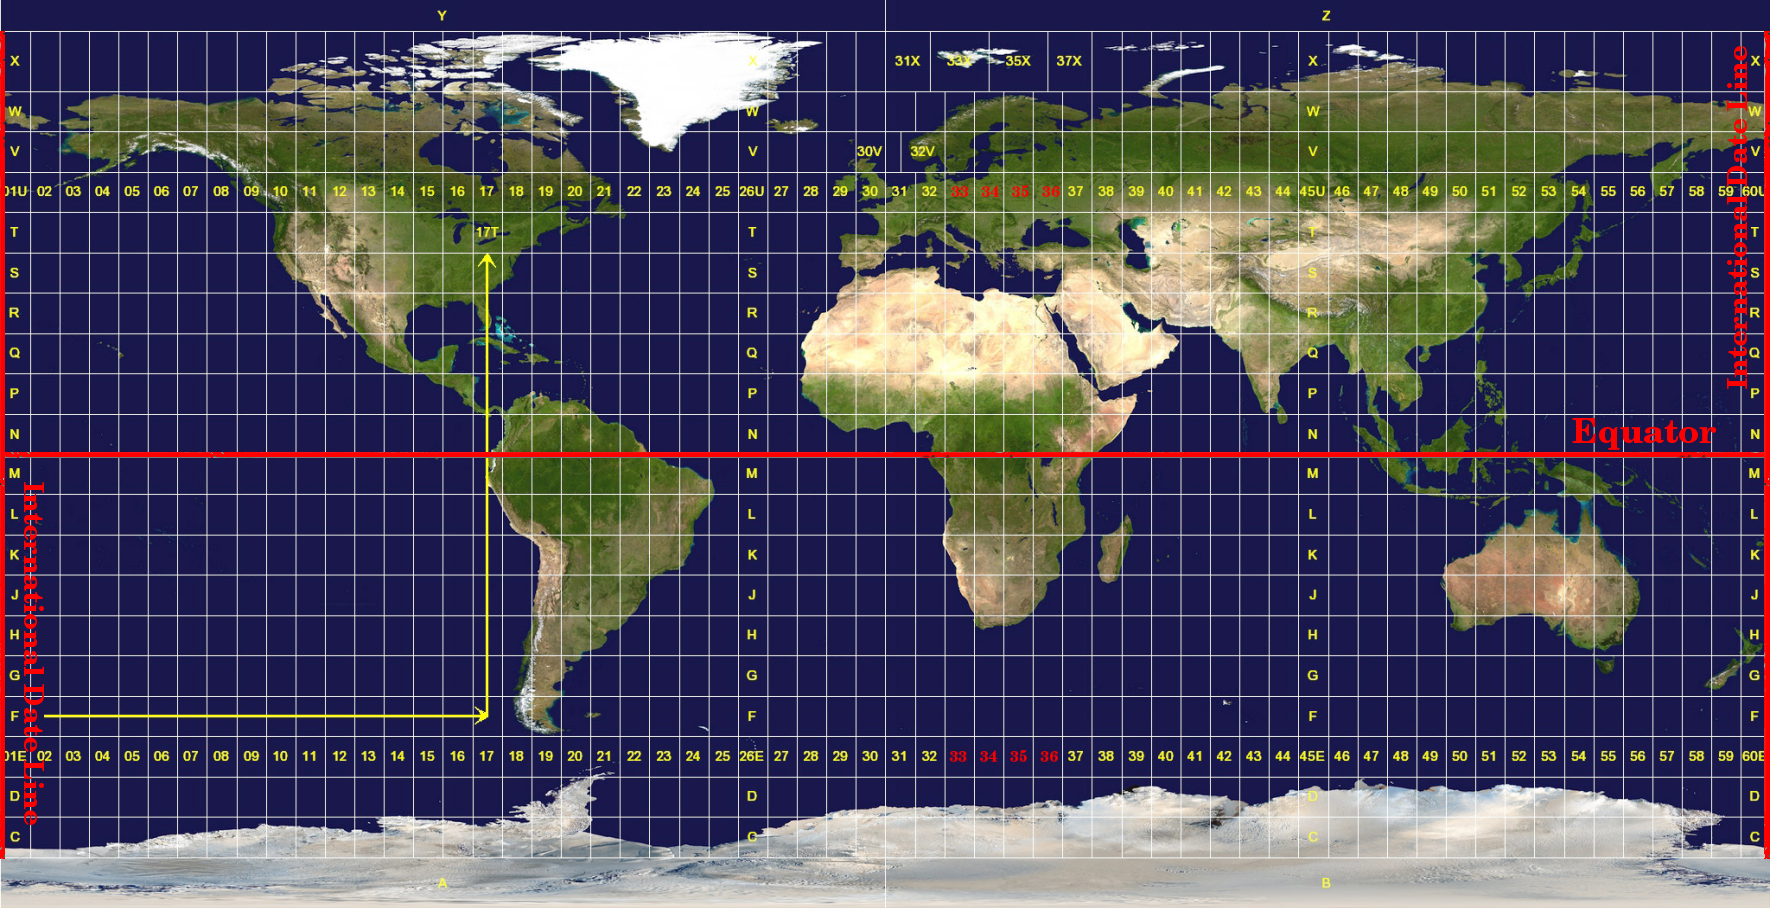
\includegraphics[width=\textwidth]{imagenes/capitulo2/2_utm2.png}
			\caption{}
		\end{subfigure}
		\caption{Sistemas de coordenadas UTM \cite{utm-nuevo}}
		\label{fig:UTM}
	\end{figure}
	
	\item \textbf{ETRS89 (\textit{European Terrestrial Reference System 1989})}. En España hasta 2008 se utilizaba el sistema oficial \textit{ED50 (European Datum 1950)}, hasta que apareció el \textit{ETRS89} y sustituyó al \textit{ED50} \cite{AsignaturaSIG}. \textit{ETRS89} es un sistema de referencia geocéntrico, muy cercano al \textit{WGS84} del GPS para ser usado no sólo en Topografía, sino en dispositivos de navegación por toda Europa. Además, está regulado por el real decreto 1071/2007 como sistema de referencia geodésico para España \cite{etrs89-nuevo}.
\end{itemize}

\begin{figure}[H]
	\centering
	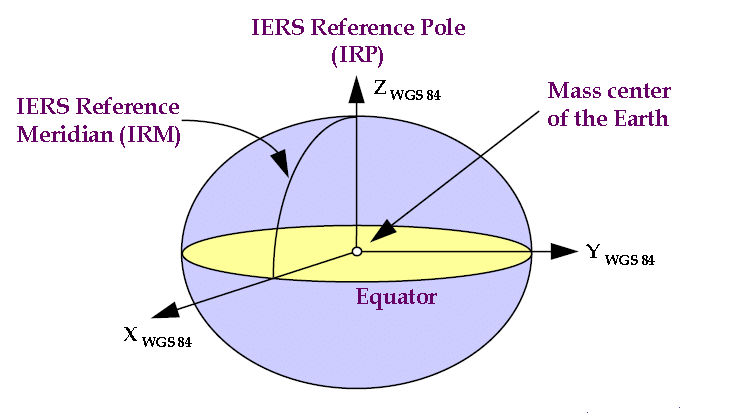
\includegraphics[height=5.35cm]{imagenes/capitulo2/Figure-36-World-Geodetic-System-1984-WGS84}
	\caption{Sistemas de coordenadas WGS84 \cite{WGS84}}
	\label{fig:WGS84}
\end{figure}

%Ambos sistemas son muy usados actualmente. Por ejemplo, \\

Tradicionalmente, la salida principal de los sistemas SIG es en formato de mapa\footnote{Un mapa ``es un conjunto de capas con información y datos, en donde los datos son codificados como alfanuméricos y contienen coordenadas que permiten ubicarlo'' \cite{congreso-ritsi}.}, lo que permite contener diferentes elementos relevantes como una leyenda (que explica lo que significan todos los símbolos utilizados), una escala (para mostrar la escala del mapa) o elementos interactivos (herramientas para hacer zoom, seleccionar capas o buscar), entre otros \cite{tesis}. Asimismo, un mapa puede estar constituido por varias capas, representadas en un orden determinado, una encima de otra. La primera capa (representada primero) generalmente se llama capa base, el resto de capas superpuestas. Las capas pueden ser muy diversas, desde fotografías aéreas, carreteras, parcelas de tierra o ríos hasta nombres de ciudades o de calles. En la figura \ref{fig:capas-mapas} podemos ver dos ejemplos de las distintas capas que puede tener un mapa \cite{VictorOlaya}.

\begin{figure}[H]
	\centering
	\begin{subfigure}[h]{0.36\textwidth} 
		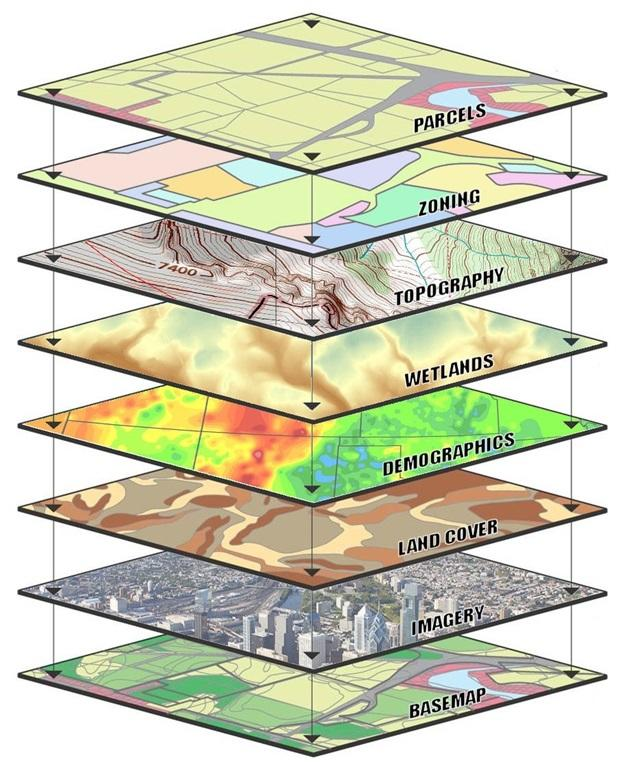
\includegraphics[width=\textwidth]{imagenes/capitulo2/2_capas-mapa-3.jpg}
		\caption{}
	\end{subfigure}       
	\begin{subfigure}[h]{0.56\textwidth} 
		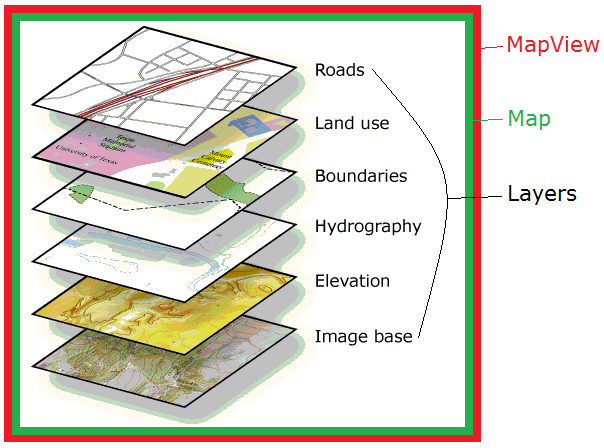
\includegraphics[width=\textwidth]{imagenes/capitulo2/2_capas-mapa-4.png}
		\caption{}
	\end{subfigure}
	\caption{Posibles capas de información en un mapa \cite{ImagenCapasMapas}}
	\label{fig:capas-mapas}
\end{figure}

En la figura \ref{fig:capas-mapas} se aprecia como cada capa aporta información relevante para la construcción del mapa, sin embargo es necesario conocer su representación. Entonces, gracias a esa información y a la Web Semántica, veremos cómo es posible transformar la capa de un mapa a instancias de una clase.

\subsection{Representación de datos geoespaciales}
\label{ch:capitulo2-representacion}

%\subsubsection{Tipo de datos}

Otra consideración importante de los mapas, es su representación. El mapa se puede representar con el modelo de datos vectorial o ráster y ambos pueden presentar la misma información de manera distinta \cite{tipos-datos-sig}:

\begin{enumerate}
	\item \textbf{Modelo de datos Vectorial}: compuesto por formas geométricas, es decir, puntos (para modelizar ocurrencias o eventos como ciudades, aeropuertos o casos de una enfermedad), líneas (para representar fenómenos estáticos como carreteras o ríos, o datos dinámicos como rutas por carreteras) o polígonos (para representar bordes como continentes, países o urbanizaciones) (figura \ref{fig:raster-vectorial}) \cite{AsignaturaSIG}. Los formatos de archivos para datos vectoriales no son tan abundantes como para los datos ráster, pero entre ellos destacamos: \textit{Shapefile (shp)} y \textit{GeoJSON}.
	
	\item \textbf{Modelo de datos Ráster}: compuesto por celdas con información (matriz regular de celdas o píxeles) en la que cada celda contiene un valor que representa información del mundo real (figura \ref{fig:raster-vectorial}). Los ráster son imágenes de satélite, fotografías aéreas digitales, imágenes digitales o mapas escaneados \cite{raster} y sus formatos de archivo son muy usados en el ámbito SIG: \textit{Tagged Image File Format (tif)}, \textit{Joint Photographic Experts Group (jpg o jpeg)} y \textit{ArcInfo ASCII (asc)}.
	
	
	
\end{enumerate}



\begin{figure}[H]
	\centering
	\begin{subfigure}[h]{0.71\textwidth} 
		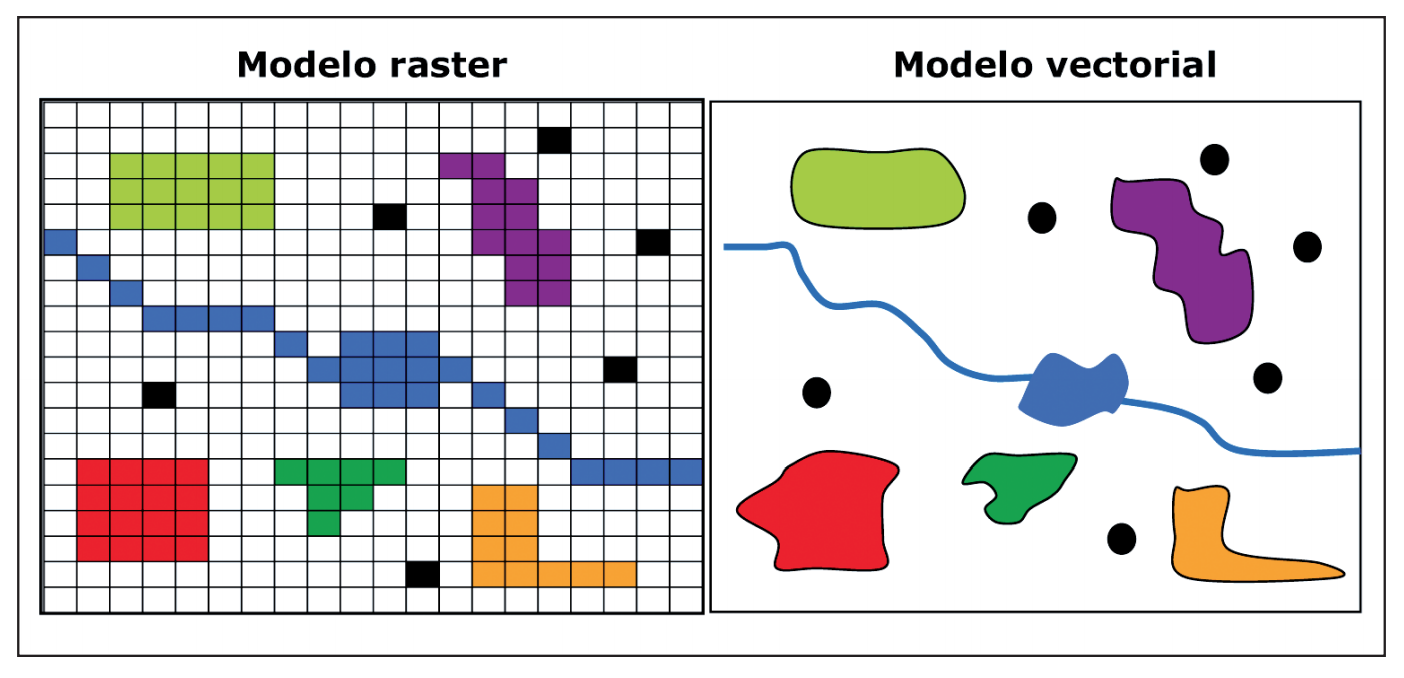
\includegraphics[width=\textwidth]{imagenes/capitulo2/raster-vectorial}
		\caption{}
	\end{subfigure}       
	\begin{subfigure}[h]{0.76\textwidth} 
		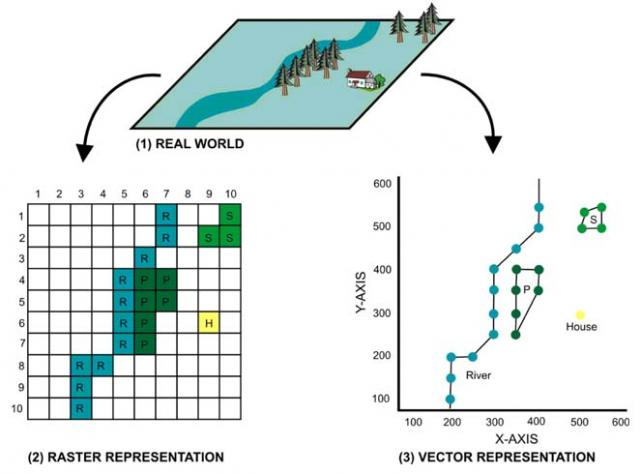
\includegraphics[width=\textwidth]{imagenes/capitulo2/raster-vector-gis-i4}
		\caption{}
	\end{subfigure}
	\caption{Representación del modelo Ráster y Vectorial \cite{imagen2-52, imagen-2.51}}
	\label{fig:raster-vectorial}
\end{figure}

Sin embargo, no es de extrañar que a veces veamos los dos modelos combinados, ya que las herramientas actuales permiten trabajar con ambos a la vez. Un ejemplo de ello es si queremos representar en un mapa con puntos las oficinas de correos de la ciudad. Además, existe una gran flexibilidad para transformar los datos de un modelo a otro.\\

%\subsubsection{Formatos}

A parte de los modelos de datos que acabamos de explicar, existen formatos estandarizados y de uso común para datos espaciales, entre ellos destacamos \textit{GML} y \textit{WKT} (usado en la prueba de concepto). La codificación \textbf{WKT} \textbf{(\textit{Well Known Text})} es una sintaxis en formato ASCII estandarizada, definida por el \textit{Open Geospatial Consortium} (OGC)\footnote{OGC es una organización internacional para crear estándares geoespaciales abiertos que define varios estándares de servicios SIG para diferentes propósitos.} para el intercambio de información espacial en formato vectorial. WKT se puede usar para representar geometrías, sistemas de referencia de coordenadas y transformaciones entre sistemas de referencia de coordenadas. Este estándar se concentra en formas de representar y manipular características simples. Las geometrías representadas usando WKT tienen las siguientes propiedades \cite{wkt-database}:

\begin{itemize}
	\item Todas las geometrías están cerradas topológicamente, lo que significa que todos los puntos que comprenden el límite de la geometría pertenecen a la geometría.
	
	\item Todas las coordenadas dentro de una geometría están en el mismo sistema de referencia de coordenadas.
\end{itemize} 

Además, está basado en un estándar que define cómo representar las geometrías de los vectores. En la figura \ref{fig:the-classes-of-geometries-in-wkt-figure-from-4} se presenta la jerarquía de clases para geometrías de características simples representadas en WKT.  Este estándar se detallará en el \texttt{capítulo \ref{ch:capitulo4}, sección \ref{ch:capitulo4-estandar} Estándar OGC para la Información Geográfica}.

\begin{figure}[H]
	\centering
	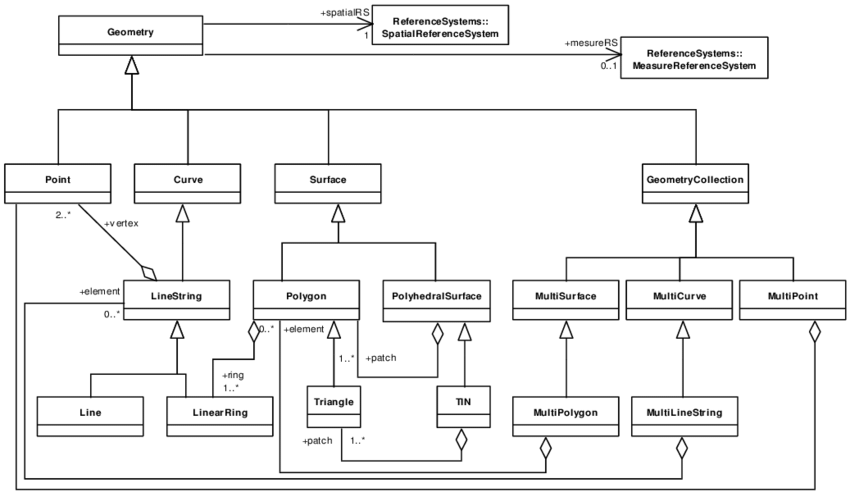
\includegraphics[width=0.9\linewidth]{imagenes/capitulo2/The-classes-of-geometries-in-WKT-figure-from-4}
	\caption{Clases de geometrías en WKT \cite{wkt-database}}
	\label{fig:the-classes-of-geometries-in-wkt-figure-from-4}
\end{figure}

En la figura \ref{fig:wkt} se aprecian los objetos que es capaz de describir WKT \cite{wkt}. Por ejemplo, la geometría de punto \texttt{POINT(37.96 23.71)} podría usarse para representar la ubicación de la ciudad de Atenas; donde 37.96 es la latitud de Atenas y 23.71 su longitud \cite{wkt-database}.

\begin{figure}[H]
	\centering
	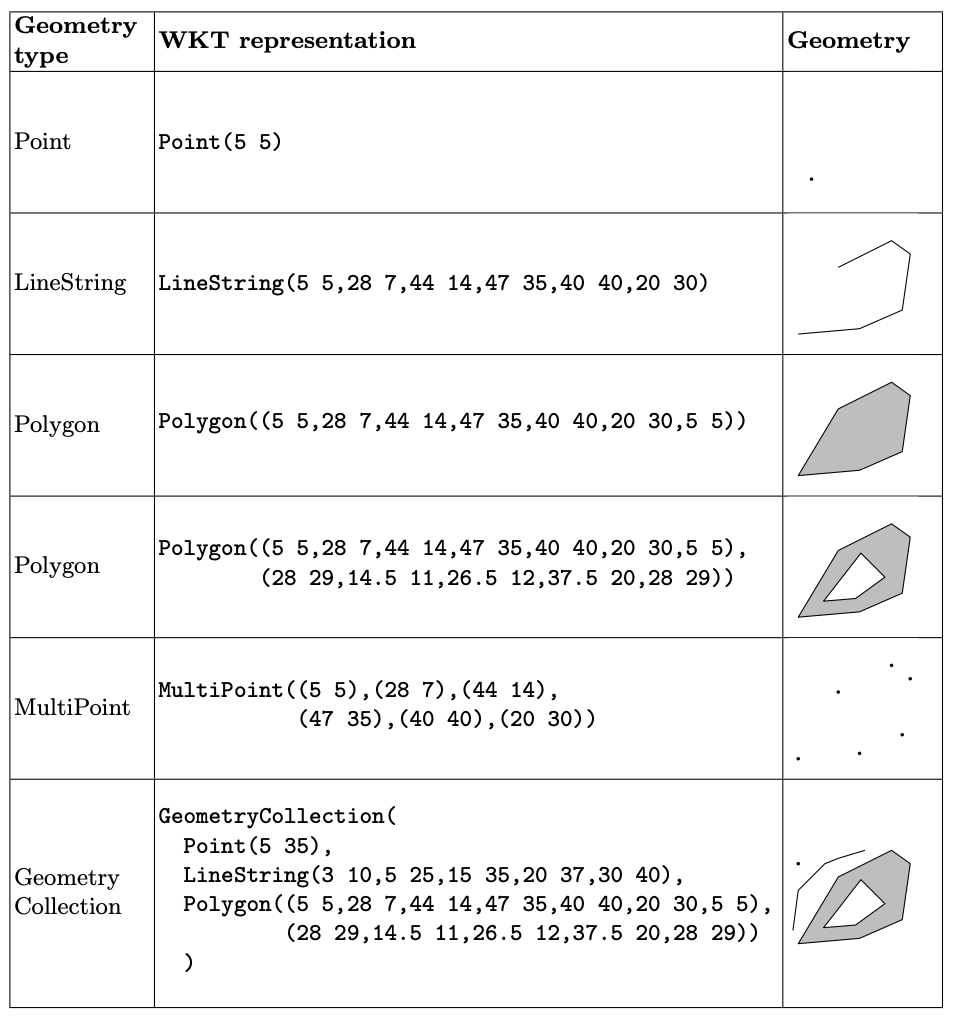
\includegraphics[width=0.93\linewidth]{imagenes/capitulo2/wkt}
	\caption{Ejemplos de geometrías representadas en WKT \cite{tesis-otro}}
	\label{fig:wkt}
\end{figure}

Por otro lado, la codificación \textbf{GML} \textbf{(\textit{Geography Markup Language})} es el estándar de codificación basado en XML más común para la representación de datos geoespaciales (figura \ref{fig:a-gml-representation-of-a-point-feature}). GML fue desarrollado por OGC y proporciona esquemas XML para definir una variedad de conceptos que son útiles en Geografía: características geográficas, geometría, sistemas de referencia de coordenadas, topología, tiempo y unidades de medida \cite{wkt-database}. Por eso, este elemento de Geografía codificado en XML (figura \ref{fig:a-gml-representation-of-a-point-feature}), es más ventajoso que WKT, ya que permite expresar más información (sistemas de referencia de coordenadas, unidades de medida, tiempo y más tipos de geometría) \cite{tesis-otro}. 


\begin{figure}[H]
	% https://www.researchgate.net/publication/266141194_Geography_20-A_mash-up_perspective
	\centering
	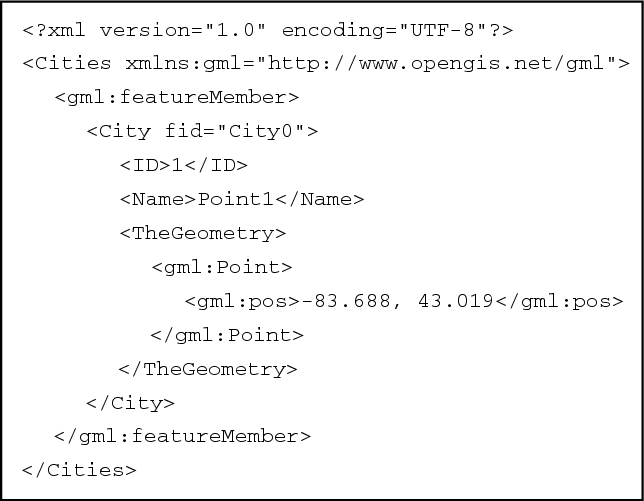
\includegraphics[width=0.71\linewidth]{imagenes/capitulo2/A-GML-representation-of-a-point-feature}
	\caption{Ejemplo de GML \cite{gml}}
	\label{fig:a-gml-representation-of-a-point-feature}
\end{figure}

%EJEMPLO DE SIG

La aparición de los SIG y las posibilidades que ofrecen para operar sobre un mapa pueden servir como impulso para la creación de diversas aplicaciones, por ejemplo, en el ámbito ambiental, la planificación de tuberías subterráneas o la gestión de los servicios de emergencia \cite{gisESRI}. Sin embargo, sigue siendo un gran problema compartir estos datos geoespaciales y utilizarlos para el desarrollo de aplicaciones SIG, no porque los datos no estén disponibles sino porque hay una gran cantidad de datos geográficos almacenados en diferentes lugares y con diferentes formatos, lo que dificulta la reutilización de datos para nuevas aplicaciones e imposibilita el intercambio de datos. De tal forma que dichas tareas son difíciles debido a la heterogeneidad de los sistemas existentes en términos de conceptos de modelado de datos, técnicas de codificación de datos y estructuras de almacenamiento. Entonces, gracias a su integración con la Web Semántica, se pueden solventar gran parte de las carencias que acabamos de comentar \cite{tesis}.

\section{?`Qué no es un SIG?}

Hasta ahora hemos visto que los SIG trabajan con Información Geográfica, no obstante existen herramientas que hacen uso y explotan de distinta manera este tipo de información, las cuales pueden incluir tecnologías o sistemas más complejos similares a los SIG pero con un enfoque totalmente distinto. Por este motivo, es imprescindible mencionar los programas de \textbf{Diseño Asistido por Ordenador (CAD)}, estas herramientas se pueden dividir básicamente en programas de dibujo 2D y de modelado 3D. Los CAD comparten características comunes con los SIG, pero no lo son \cite{VictorOlaya}, ya que aparte de ser muy usados en áreas como la arquitectura para crear planos en 3D, presentan diferencias con los SIG \cite{sig-cad}:

\begin{itemize}
	
	\item Los SIG tienen un abanico infinito de posibilidades (agricultura, hidrología, teledetección, arqueología). Sin embargo, un CAD está limitado a la producción de planos, centrándose sobre todo en el ámbito de generación de planos para ingeniería (ingeniería civil y urbanismo), instalaciones mecánicas, diseño de plantas o arquitectura.
	
	\item En un SIG siempre debemos trabajar con información georreferenciada, es decir, debemos tener esta información ubicada en el espacio y vinculada a un sistema de referencia espacial.
	
	%\item Un CAD permite el diseño informatizado de elementos muy diversos: desde la carrocería de un avión (tarea poco relacionada con los SIG) hasta el diseño de una urbanización (mayor relación con los SIG).
	
	%\item Un CAD no está pensado para gestionar datos de una superficie como la de un país o continente.
	
	\item Un SIG refleja la realidad y un CAD diseña algo que no existe aún, por tanto con un SIG podemos realizar operaciones que nos ayuden a tomar decisiones, lo que con un CAD no sería posible.
	
	\item Un dato SIG se almacena como un dato geográfico complejo, mientras que un dato CAD se almacena como un \textit{dibujo} (figura \ref{fig:c4nmjdnwcaaoub7}).
	
	\item En un CAD lo habitual es trabajar con un único fichero que contenga distinta información, mientras que en un SIG tradicionalmente se trabaja con un fichero por cada tipo de geometría.
	
\end{itemize}


%\begin{figure}[H]
%	\centering
%	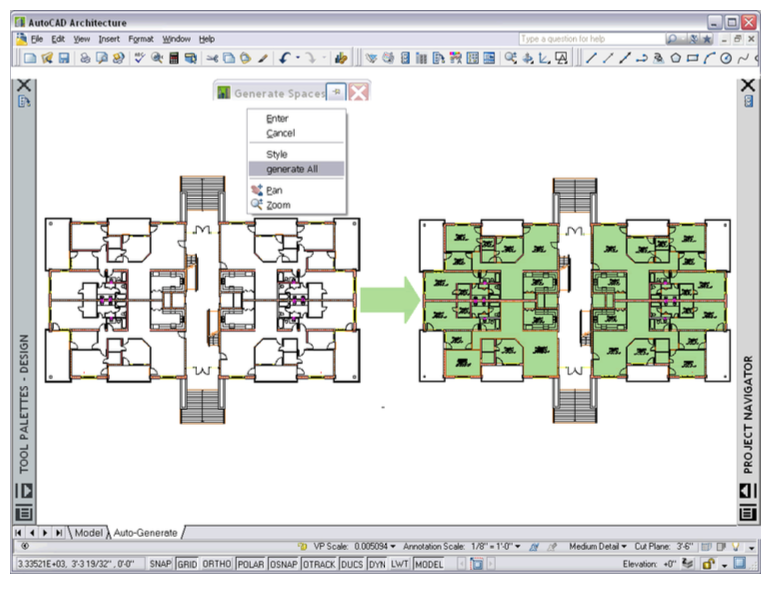
\includegraphics[height=6.5cm]{imagenes/capitulo2/2_CAD.png}
%	\caption{Entorno de trabajo de una aplicación CAD \cite{VictorOlaya}}
%	\label{fig:CAD}
%\end{figure}

\begin{figure}[H]
	\centering
	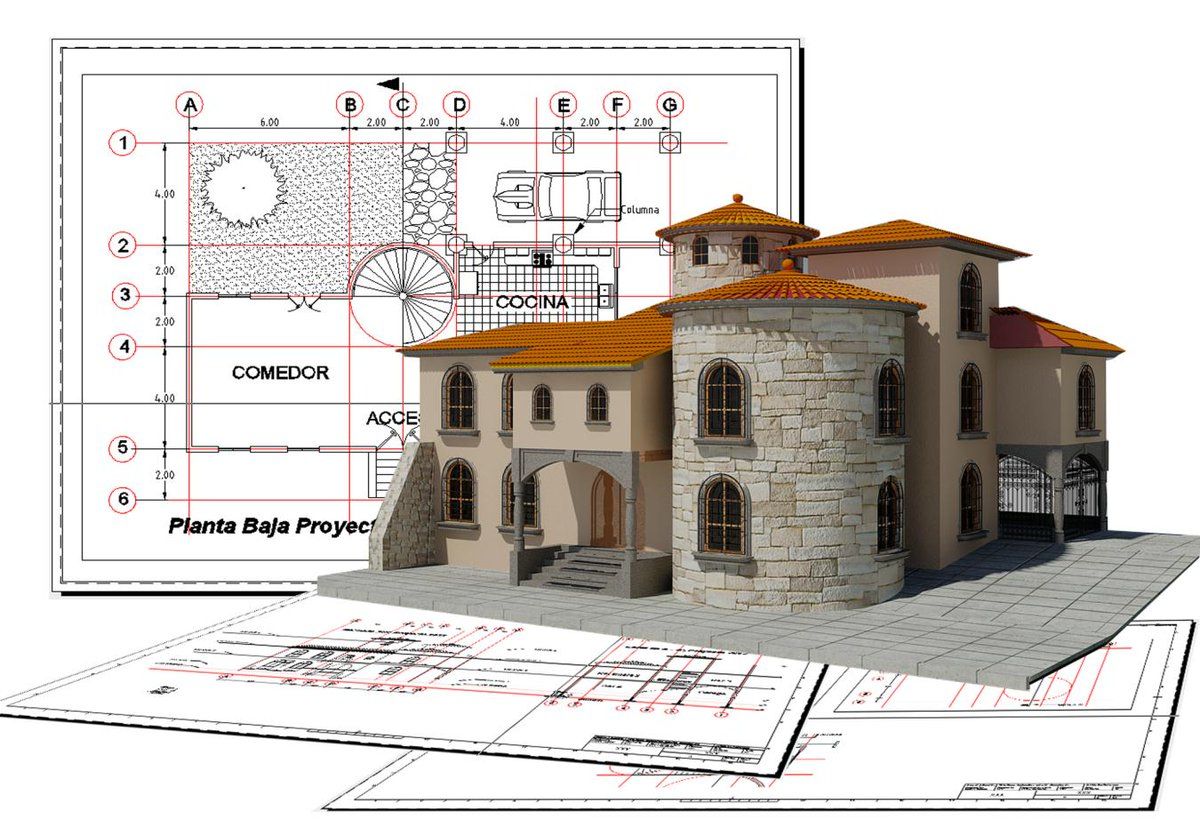
\includegraphics[width=0.75\linewidth]{imagenes/capitulo2/C4nMJdNWcAAoub7}
	\caption{Entorno de trabajo de una aplicación CAD  \cite{sig-cad}}
	\label{fig:c4nmjdnwcaaoub7}
\end{figure}




\section{Tipos de software SIG}

Dentro de los tipos de software disponibles para la manipulación de datos geoespaciales, existen sistemas de software SIG de escritorio tanto comerciales como \textit{open-source}, es decir, libres y no libres. Dentro de los softwares no libres, podemos ubicar los softwares no comerciales, como los creados por empresas u organismos gubernamentales, algunos de los cuales son accesibles desde su plataforma Web. Por otro lado, los diferentes proveedores tienen sus propios diseños de software propietario, modelos de datos y estructuras de almacenamiento de bases de datos. Por lo tanto, las bases de datos geográficas basadas en estos diseños no pueden comunicarse sin la conversión de datos. Entonces, para intercambiar información y compartir recursos entre sistemas heterogéneos, se deben desarrollar herramientas de conversión para transferir datos de un formato a otro y así mejorar dicha acesibilidad \cite{libro-gis}. \\

% Es improbable que todas las aplicaciones GIS utilicen el mismo software. Los diferentes proveedores tienen sus propios diseños de software propietario, modelos de datos y estructuras de almacenamiento de bases de datos. Por lo tanto, las bases de datos geográficas basadas en estos diseños no pueden comunicarse sin la conversión de datos. Para intercambiar información y compartir recursos de geo-bases de datos computacionales entre sistemas heterogéneos, se deben desarrollar herramientas de conversión para transferir datos de un formato a otro. Además, estas diversas estructuras de bases de datos SIG de escritorio hacen que el intercambio de datos remoto y el intercambio sean más difíciles debido a la accesibilidad limitada y la conversión de datos requerida.\\

Por otra parte, también podemos encontrar otro tipo de software relacionado con la posibilidad de compartir datos a través de la Web, conocidos como Web SIG (\textit{Esri’s ArcGIS Server} o \textit{MapInfo’s MapExtreme}). Estos programas ofrecen mejores herramientas para compartir datos en la Web, no obstante tienen los mismos problemas de los diseños del software propietario, los modelos de datos y las estructuras de almacenamiento de bases de datos \cite{libro-gis}. El intercambio de datos, facilitado por los avances en las tecnologías de red, se ve obstaculizado por la incompatibilidad de la variedad de modelos y formatos de datos utilizados en diferentes sitios. \\

En la tabla \ref{softwaresSIG} mostramos los software SIG más usados a nivel nacional, sin olvidarnos de que cada país u organismo puede hacer uso de otros.

%Internet GIS o Web GIS crea un entorno único para compartir datos geoespaciales. Hay muchos programas de Internet GIS o Web GIS disponibles para compartir datos a través de la Web, como Esri’s ArcGIS Server, Intergraph’s GeoMedia WebMap, MapInfo’s MapExtreme, AutoDesk’s MapGuide, GE SmallWorld’s Internet Application Server y ER Mapper’s Image Web Server.\\

%Aunque estos programas de Internet GIS ofrecen mejores herramientas para compartir datos en la Web, también tienen los problemas de los diseños de software propietario, los modelos de datos y las estructuras de almacenamiento de bases de datos. El intercambio de datos, facilitado por los avances en las tecnologías de red, se ve obstaculizado por la incompatibilidad de la variedad de modelos y formatos de datos utilizados en diferentes sitios.\\

\begin{table}[H]
	\centering
	\caption{Tipos de Software SIG}
	\label{softwaresSIG}
	\begin{tabular}[b]{|m{2.44cm}||m{8.69cm}|}
		\hline
		
		\cellcolor[HTML]{EFEFEF} \centering \textbf{Software} & \cellcolor[HTML]{EFEFEF} \textbf{Descripción} \\ \hline \hline
		
		% \centering \large{\xmark}
		% \large{\cmark}
		
		\centering \href{https://www.arcgis.com/}{\underline{ESRI ArcGIS}} & Conjunto de productos de software no libre SIG producido y comercializado por ESRI \\ \hline
		
		\centering \href{https://qgis.org/es/site/}{\underline{QGIS}} & Software libre de la fundación OSGeo para plataformas GNU/Linux, Unix, MacOS, Microsoft Windows y Android, que permite manejar formatos ráster y vectoriales a través de las bibliotecas GDAL y OGR \\ \hline
		
		\centering \href{http://www.saga-gis.org/}{\underline{SAGA GIS}} & Programa libre que se utiliza para editar datos espaciales, desarrollado por el Dep. de Geografía Física de la Univ. de Göttingen (Alemania). Actualmente mantenido por una comunidad de desarrolladores \\ \hline
		
		%\centering \href{https://clarklabs.org/terrset/}{\underline{TerrSet}} & Software no libre geoespacial integrado para monitorear y modelar el sistema terrestre para el desarrollo sostenible, ofrece el conjunto más amplio de herramientas geoespaciales de la industria \\ \hline
		
		\centering \href{https://grass.osgeo.org}{\underline{GRASS GIS}} & Software libre SIG bajo licencia GPL, que puede soportar información tanto ráster como vectorial y posee herramientas de procesado digital de imágenes \\ \hline
		
		\centering \href{http://www.gvsig.com/es}{\underline{gvGIS}} & Proyecto de desarrollo de software libre para SIG, impulsado por el gobierno regional de la Comunidad Valenciana (Generalidad Valenciana) de España \\ \hline
		
		%\centering \href{http://mapas.xunta.gal/portada}{\underline{SITGA}} & Creada por un organismo gubernamental para los datos espaciales de Galicia, cuenta con los servicios básicos de OGC y otras funcionalidades \\ \hline
		
	\end{tabular}
\end{table}


 %Además de usar QGIS, también haremos uso de otras herramientas relacionadas con la Web Semántica y que nos permiten integrar Información Geográfica.

%Además, como hemos ido viendo a lo largo del capítulo, existen miles de aplicaciones en el mundo de los SIG, los cuales caen fuera del ámbito de este trabajo, sin embargo, nos centraremos en general en el análisis de los MDT y, en particular, en su aplicación para obtener el mapa de sombras. De todos modos, comentaremos algunos estudios y/o aplicaciones adicionales. En el siguiente capítulo, profundizamos sobre todos estos temas mencionados.


\section{Conclusiones}

Este capítulo ha introducido los SIG como a un término amplio que hace referencia a una amplia familia de estándares, tecnologías y herramientas de software para almacenar, editar, analizar, mostrar e integrar datos espaciales. Dichos datos espaciales necesitan hacer uso de un sistema de referencia con el que poder expresar la situación de un punto dado; entre los sistemas que existen en la actualidad debemos destacar \textit{UTM} y \textit{WGS4}. No obstante, en España se utiliza el oficial en Europa, \textit{ETRS89 (European Terrestrial Reference System 1989)}. Entre los SIG de código abierto, es importante subrayar que QGIS es a día hoy el software libre con más proyección. Además este software nos permitirá obtener la codificación WKT para la representación de las geometrías, debido a que este formato es el empleado en la representación de la estructura para los datos geográficos de la Web Semántica en las consultas con GeoSPARQL.

%Este capítulo ha introducido los SIG como a un término amplio que hace referencia a una amplia familia de estándares, tecnologías y herramientas de software para almacenar, editar, analizar, mostrar e integrar datos espaciales. Dichos datos espaciales necesitan hacer uso de un sistema de referencia con el que poder expresar la situación de un punto dado; entre los sistemas que existen en la actualidad debemos destacar \textit{UTM} y \textit{WGS4}. No obstante, en España se utiliza el oficial en Europa, \textit{ETRS89 (European Terrestrial Reference System 1989)}, y será el que usen nuestros datos geográficos. Respecto los datos geoespaciales, vamos a coger datos en formato \textit{Shapefiles} procedentes del Instituto de Estadística y Cartografía de Andalucía, en donde nos centraremos en las capas de edificaciones (geometría de polígonos), curvas de nivel (geometría de líneas) y puntos de cota (geometría de puntos) procedentes de Ogíjares (Granada). Entre los SIG de código abierto, es importante subrayar que QGIS es a día hoy el software libre con más proyección. Por eso mismo y por tener conocimientos en el manejo de este programa, voy hacer uso de él para obtener la información relevante de los \textit{Shapefile} a hojas de cálculo y para ver su representación. Además este software nos permitirá obtener la codificación WKT para la representación de las geometrías, debido a que este formato es el empleado en la representación de la estructura para los datos geográficos de la Web Semántica en las consultas con GeoSPARQL.
